\documentclass{article}

\usepackage{fancyhdr} % Required for custom headers
\usepackage{lastpage} % Required to determine the last page for the footer
\usepackage{extramarks} % Required for headers and footers
\usepackage[usenames,dvipsnames]{color} % Required for custom colors
\usepackage{graphicx} % Required to insert images
\usepackage{listings} % Required for insertion of code
\usepackage{courier} % Required for the courier font
\usepackage{lipsum} % Used for inserting dummy 'Lorem ipsum' text into the template
\usepackage{hyperref}
\usepackage{multirow}
\usepackage{tabularx}
\usepackage{longtable}
\usepackage{listings}
\usepackage{subfigure}
\usepackage{afterpage}
\usepackage{amsmath,amssymb}            
\usepackage{rotating}  
\usepackage{fancyhdr}
\usepackage{graphicx}
\usepackage{amsthm}
\usepackage[scriptsize]{caption} 
\hyphenation{a-gen-tiz-za-zio-ne}
% Margins
\topmargin=-0.45in
\evensidemargin=0in
\oddsidemargin=0in
\textwidth=6.5in
\textheight=9.0in
\headsep=0.25in

\linespread{1.1} % Line spacing

% Set up the header and footer
\pagestyle{fancy}
\lhead{\hmwkAuthorName} % Top left header
\chead{\hmwkClass\ (\hmwkClassInstructor\ \hmwkClassTime): \hmwkTitle} % Top center head
\rhead{\firstxmark} % Top right header
\lfoot{\lastxmark} % Bottom left footer
\cfoot{} % Bottom center footer
\rfoot{Page\ \thepage\ of\ \protect\pageref{LastPage}} % Bottom right footer
\renewcommand\headrulewidth{0.4pt} % Size of the header rule
\renewcommand\footrulewidth{0.4pt} % Size of the footer rule

\setlength\parindent{0pt} % Removes all indentation from paragraphs

\usepackage{listings}
\usepackage{color}

\definecolor{dkgreen}{rgb}{0,0.6,0}
\definecolor{gray}{rgb}{0.5,0.5,0.5}
\definecolor{mauve}{rgb}{0.58,0,0.82}

\lstset{frame=tb,
  language=Java,
  aboveskip=3mm,
  belowskip=3mm,
  showstringspaces=false,
  columns=flexible,
  basicstyle={\small\ttfamily},
  numbers=none,
  numberstyle=\tiny\color{gray},
  keywordstyle=\color{blue},
  commentstyle=\color{dkgreen},
  stringstyle=\color{mauve},
  breaklines=true,
  breakatwhitespace=true
  tabsize=3
}

%----------------------------------------------------------------------------------------
%	DOCUMENT STRUCTURE COMMANDS
%	Skip this unless you know what you're doing
%----------------------------------------------------------------------------------------

% Header and footer for when a page split occurs within a problem environment
\newcommand{\enterProblemHeader}[1]{
\nobreak\extramarks{#1}{#1 continued on next page\ldots}\nobreak
\nobreak\extramarks{#1 (continued)}{#1 continued on next page\ldots}\nobreak
}

% Header and footer for when a page split occurs between problem environments
\newcommand{\exitProblemHeader}[1]{
\nobreak\extramarks{#1 (continued)}{#1 continued on next page\ldots}\nobreak
\nobreak\extramarks{#1}{}\nobreak
}




%----------------------------------------------------------------------------------------
%	NAME AND CLASS SECTION
%----------------------------------------------------------------------------------------

\newcommand{\hmwkTitle}{Design Pattern} % Assignment title
\newcommand{\hmwkDueDate}{Martedi,\ Aprile 15,\ 2014} % Due date
\newcommand{\hmwkClass}{Ingegneria del Software 1} % Course/class
\newcommand{\hmwkClassTime}{} % Class/lecture time
\newcommand{\hmwkClassInstructor}{} % Teacher/lecturer
\newcommand{\hmwkAuthorName}{} % Your name

%----------------------------------------------------------------------------------------
%	TITLE PAGE
%----------------------------------------------------------------------------------------

\title{
\vspace{2in}
\textmd{\textbf{\hmwkClass:\ \hmwkTitle}}\\
\normalsize\vspace{0.1in}\small{Due\ on\ \hmwkDueDate}\\
\vspace{0.1in}\large{\textit{\hmwkClassInstructor\ \hmwkClassTime}}
\vspace{3in}
}

\author{\textbf{\hmwkAuthorName}}
\date{} % Insert date here if you want it to appear below your name

%----------------------------------------------------------------------------------------

\begin{document}

\maketitle

%----------------------------------------------------------------------------------------
%	TABLE OF CONTENTS
%----------------------------------------------------------------------------------------

%\setcounter{tocdepth}{1} % Uncomment this line if you don't want subsections listed in the ToC

\newpage
\tableofcontents
\newpage



%----------------------------------------------------------------------------------------
\section{Introduction}


\section{Creational Patterns Theory}
Inside the class of the creational patterns we can distinguish between two main pattern:
\begin{itemize}
\item \textbf{class creational pattern} uses inheritance to change how the different classes are intantiated (Singleton~\ref{Singleton}).
\item \textbf{object creational pattern} delegate the instantiation of the object to another object.
\end{itemize}
The object creational pattern become important when it is necessary to compose a smaller set of composed behavior into complex one. Thus, creating an object with a particular behavior is more complex then simply instantiating a new class.

\subsection{Singleton}
\label{Singleton}
\subsubsection{Goal}
Guarantee that only \textbf{one instance} of a specific class is created and allow to create that instance.

\subsubsection{Structure}
\begin{figure}[h!]
  \centering
    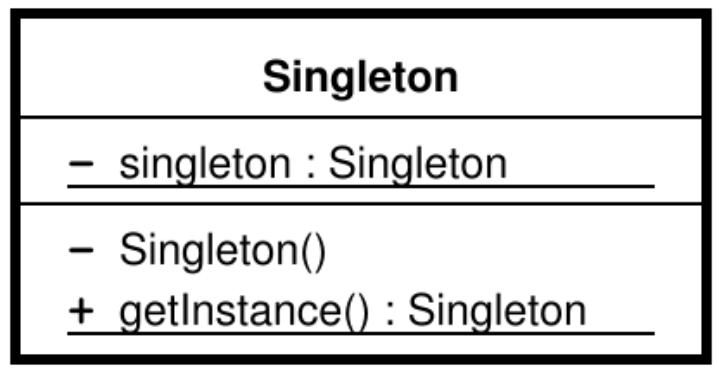
\includegraphics[width=0.3\textwidth]{Img/SingletonUML.png}
     \caption{Singleton UML}
     \label{SingletonUML}
\end{figure}
General idea: make the class ensuring that \textbf{only} one instance is creating. The idea is to make the class able to intersect creation of new objects and to provide an easy way to access the instance.

\subsubsection{Implementation}
The class which must be singleton (in this case named as $Singleton$) has
\begin{itemize}
\item a \textbf{static} attribute $singleton$ of type $Singleton$
\item a \textbf{private} constructor (in this case $Singleton()$) which could have also parameters
\item a \textbf{public} and \textbf{static} method $getInstance()$ which returns the instance of the singleton class. The method $getInstance$ is the only way to instantiate the object and thus can guarantee the access of the unique copy referenced by the $static$ attribute singleton. 
\end{itemize}


\subsubsection{Examples}
\textbf{Printer spooler}\\
 Although there can be many printers in a system, there should be only one printer spooler.
 
 \textbf{File system, Window manager}\\
 There should be only one file system and one window manager.
 
\subsubsection{When to use it}
\begin{itemize}
\item when it is necessary to instantiate  a class exactly once (the class must be accessible to the client from a well known access point).
\item when it is necessary to control the access to the instance (it is possible to control $who$ and $when$ can access the instance).
\item it can reduce the number of instances of an object in the system
\item allows the refinement of the class and provides a way to configure the application to get the instance of the class you need at run-time
\item it allows using a similar approach to control the number of instances of a class at run-time
\end{itemize}

\subsection{Prototype}

\subsection{Abstract Factory (Kit)}
\subsubsection{Goal}
The goal is to create an interface which allows \textbf{to create families} of related or dependent objects, \textit{without specifying} their concrete classes. 

\subsubsection{Structure}

\begin{figure}[h!]
  \centering
    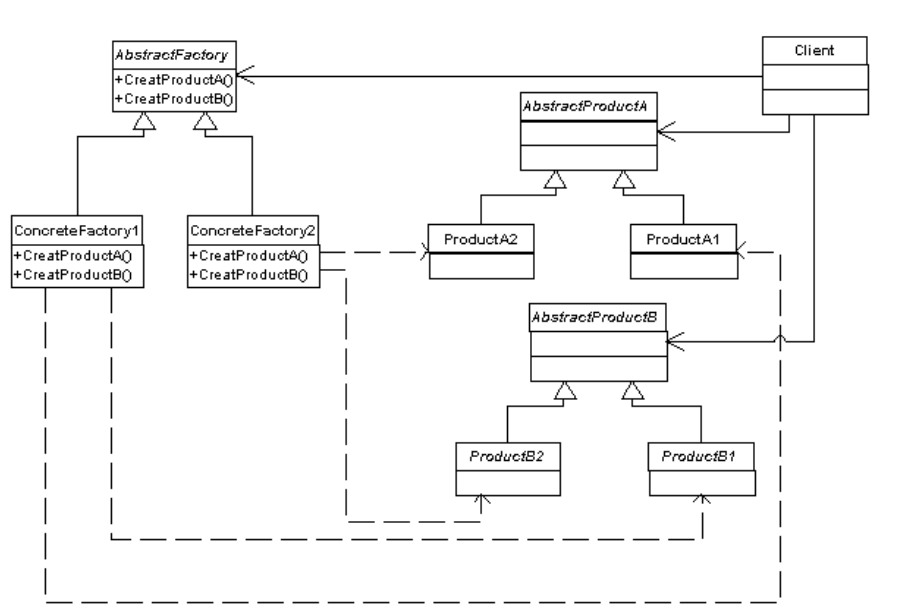
\includegraphics[width=0.8\textwidth]{Img/AbstractFactoryUML.png}
     \caption{Abstract Factory UML.}
     \label{AbstractFactoryUML}
\end{figure}

Using this pattern an abstract framework (factory) is defined, which allows to create objects that follow a general pattern. At run-time the abstract factory is paired with any concrete factory that allows to create the objects that follow the concrete pattern. In other words, the Abstract Factory is a super-factory which creates other factories (Factory of factories). The UML of Figure~\ref{AbstractFactoryUML} is composed by the following classes:
\begin{itemize}
\item \emph{AbstractFactory}: is an abstract class (see the italic style of the text), which declares the interface for the operations that allows to create \emph{abstract} products
\item \emph{ConcreteFactory}: are the concrete classes that allows to create \emph{concrete} products (Note the hierarchical relation between the AbstractFactory and the ConcreteFactory). Each product is a family of related dependent objects AbstractProductA and AbstractProductB, and in particular, for the ConcreteFactory1 the products are ProductA1 and ProductB1, while for the ConcreteFactory2 the products are ProductA2 and ProductB2 (Note the uses relation between the Factories and the products).
\item \emph{AbstractProduct}:  declares an abstract product which can be aggregated to other products using appropriate factories
\item \emph{ConcreteProduct}: are  concrete products which extends  particular abstract products.
\item \emph{Client}: instantiate a specific ConcreteFactory (depending on its necessities) to obtain specific products.
\end{itemize}

Note: usually only a single instance of a ConcreteFactory class is created at run-time. The AbstractFactory defers the creation of products to the ConcreteFactories.

\subsubsection{Implementation}
\begin{itemize}
\item \emph{AbstractFactory} only declare the interface for the creating the products
\item \emph{ConcreteFactory} are \emph{singleton}. A \emph{factory method} is defined for each product. 
\end{itemize}


\subsubsection{Examples}
\emph{Window Interface}\\
Consider a user interface that must support multiple devices, such as laptops, cellphones. Different interfaces must be creating depending on the device which runs the application (e.g., different type of scroll bars, windows, buttons). To be portable, the application should not be hard-coded to a particular look and feel. The instantiation and the designing new look-and-feels must be easy. The example is inspired by~\cite{gamma1994design}.



\subsubsection{Pro and Cons}
\begin{itemize}
\item it requires a concrete factory subclass for each product even if the families differ only slightly
\item if many families are possible think about using a \emph{prototype pattern} inside the factory (You can store classes inside a concrete factory that create the various concrete products in variables, much like prototypes).
\item AbstractFactory usually define a \emph{different operation} for each kind of product it is possible to create, i.e., for each product there is a signature in the AbstractFactory Interface. This implies that \emph{to add a new product} you must add the \emph{signature in the abstract factory} and all the sub Factory-classes. A \textbf{more flexible} but \textbf{less safe} design is to add a parameter in the operations to create objects. This parameter specifies the object to be created (e.g., an enum).
\item All the products are returned to the client as abstract interfaces to the product. The client is not able to make safe assumption on the type of the product.
\end{itemize}



\subsection{Builder}
\subsubsection{Goal}
Separate the construction of a complex object from its representation, so that the same construction process can create different representations.

\subsubsection{Motivation}



\subsection{Factory Method (Virtual Constructor)}
\subsubsection{Goal}
Define an interface for creating an object, but let sub-classes decide which class to instantiate.




\section{Creational Patterns Exercises}
\subsection{Singleton}

\subsubsection{EagerSingleton}
\begin{lstlisting}
package creationalpatterns.singleton;

/**
 * 
 * @author claudio menghi
 * The singleton class ensures that only a unique instance of the class can be ever created
 * Note that 
 * -	the object is created and instantiated before its first use
 * -	if the object is big and it is not used a lot of memory is occupied and not used
 * -	it is thread safe
 */
public class EagerSingleton {

	/**
	 * contains the unique instance of the {@link EagerSingleton} class
	 * if the object is big it can occupy a lot of memory if not used
	 */
	private static EagerSingleton uniqueInstance=new EagerSingleton();
	
	/**
	 * The constructor of the {@link EagerSingleton} class is hided (either private or protected). 
	 * If protected it is possible to call the constructor from the subclasses 
	 */
	private EagerSingleton(){
		
	}
	
	/**
	 * returns the pointer to the unique instance of the class
	 * @return the pointer to the unique instance of the {@link EagerSingleton} class
	 */
	public static EagerSingleton getInstance(){
		return uniqueInstance;
	}
}
\end{lstlisting}


\subsubsection{Lazy Singleton}

\begin{lstlisting}
package creationalpatterns.singleton;

/**
 * @author Claudio Menghi
 * The singleton class ensures that only a unique instance of the class can be ever created
 * Note that 
 * -	the object is instantiated only when needed
 * -	it does not occupy additional memory as the {@link EagerSingleton}
 * -	it is NOT THREAD safe -> it does not work for multithreads applications
 */
public class LazySingleton {
	
	/**
	 * contains the unique instance of the {@link LazySingleton} class
	 */
	private static LazySingleton uniqueInstance;
	// other attributes
	
	/**
	 * The constructor of the {@link LazySingleton} class is hided (either private or protected). 
	 * If protected it is possible to call the constructor from the subclasses 
	 */
	private LazySingleton(){
		// initialization of other attributes
	}
	
	/**
	 * returns the pointer to the unique instance of the class
	 * @return the pointer to the unique instance of the {@link LazySingleton} class
	 */
	public static LazySingleton getInstance(){
		
		// if the instance has not already been created,  the new instance is created
		if(uniqueInstance==null){
			uniqueInstance=new LazySingleton();
		}
		// the instance is returned
		return uniqueInstance;
	}	
}
\end{lstlisting}


\subsubsection{Synchronized Lazy Singleton}
\begin{lstlisting}
/**
 * @author Claudio Menghi
 * The {@link SynchronizedLazySingleton} alters the {@link LazySingleton} 
 * to guarantee the correct behavior of the {@link LazySingleton} in case of multithreading 
 */
public class SynchronizedLazySingleton {
	/**
	 * contains the unique instance of the {@link SynchronizedLazySingleton} class
	 */
	private static SynchronizedLazySingleton uniqueInstance;
	
	private SynchronizedLazySingleton(){
		// costruttore
	}
	
	/**
	 * returns the pointer to the unique instance of the class. The syncronized attribute guarantees the correct behaviour
	 * is a multithreading environment
	 * @return the pointer to the unique instance of the {@link SynchronizedLazySingleton} class
	 */
	public static synchronized SynchronizedLazySingleton getInstance(){
		// metodi synchronized possono essere inefficienti
		if (uniqueInstance == null){
			uniqueInstance = new SynchronizedLazySingleton();
		}
		return uniqueInstance;
			
	}
}
\end{lstlisting}

\subsubsection{Enum Singleton}

\begin{lstlisting}
package creationalpatterns.singleton;

/**
 * Metodo alternativo e thread safe. Non supporta ereditarieta'
 * @author claudio menghi
 */
public enum EnumSingleton {
	INSTANCE;
	public static EnumSingleton getInstance(){
		return INSTANCE;
	}
}
\end{lstlisting}

\clearpage
% ---- Bibliography ----




\addcontentsline{toc}{chapter}{Bibliography}
\bibliographystyle{alpha}
\bibliography{DesignPatterns}
\nocite{*}


\end{document}

